\documentclass[12pt, a4paper]{book}
\usepackage[T1]{fontenc}
\usepackage[utf8]{inputenc}
\usepackage[charter, cal=cmcal]{mathdesign}
\usepackage[scaled=0.92]{helvet}
\usepackage{geometry}
\geometry{a4paper, top=30mm, bottom=30mm, inner=32mm, outer=25mm}
\usepackage{amsmath, amssymb}
\usepackage[version=4]{mhchem}
\usepackage[dvipsnames,svgnames,table]{xcolor}
\usepackage{tikz}
\usetikzlibrary{arrows.meta, positioning, calc, backgrounds}
\usepackage{pgfplots}
\pgfplotsset{compat=1.18}
\usepackage{tcolorbox}
\tcbuselibrary{skins, breakable}
\usepackage{titlesec}
\usepackage{fancyhdr}
\usepackage{enumitem}
\usepackage{booktabs}
\usepackage{array}
\usepackage{parskip}
\usepackage{siunitx}
\usepackage[colorlinks=true, linkcolor=BrickRed, urlcolor=NavyBlue]{hyperref}

\definecolor{JourneyColor}{HTML}{1A5276}
\definecolor{ModuleColor}{HTML}{2E86C1}
\definecolor{PuzzleColor}{HTML}{145A32}
\definecolor{DiscoveryColor}{HTML}{B7950B}
\definecolor{WarningColor}{HTML}{C0392B}
\definecolor{ProblemColor}{HTML}{4A235A}
\definecolor{ReflectColor}{HTML}{117A65}
\definecolor{HistoryColor}{HTML}{6E2F1A}
\definecolor{IonicColor}{HTML}{922B21}
\definecolor{LatticeColor}{HTML}{1A5276}

\newtcolorbox{puzzlebox}[1][]{enhanced,breakable,
  colback=PuzzleColor!6,colframe=PuzzleColor,fonttitle=\bfseries\sffamily,
  title={The Puzzle},attach boxed title to top left={yshift=-2mm,xshift=6mm},
  boxed title style={colback=PuzzleColor},borderline west={3pt}{0pt}{PuzzleColor},#1}
\newtcolorbox{discoverybox}[1][]{enhanced,breakable,
  colback=DiscoveryColor!8,colframe=DiscoveryColor,fonttitle=\bfseries\sffamily,
  title={Discovery},attach boxed title to top left={yshift=-2mm,xshift=6mm},
  boxed title style={colback=DiscoveryColor},borderline west={3pt}{0pt}{DiscoveryColor},#1}
\newtcolorbox{problembox}[1][]{enhanced,breakable,
  colback=ProblemColor!5,colframe=ProblemColor,fonttitle=\bfseries\sffamily,
  title={Problems},attach boxed title to top left={yshift=-2mm,xshift=6mm},
  boxed title style={colback=ProblemColor},borderline west={3pt}{0pt}{ProblemColor},#1}
\newtcolorbox{deepbox}[1][]{enhanced,breakable,
  colback=JourneyColor!5,colframe=JourneyColor,fonttitle=\bfseries\sffamily,
  title={Deep Problems},attach boxed title to top left={yshift=-2mm,xshift=6mm},
  boxed title style={colback=JourneyColor},borderline west={4pt}{0pt}{JourneyColor},#1}
\newtcolorbox{historybox}[1][]{enhanced,breakable,
  colback=HistoryColor!7,colframe=HistoryColor!60,fonttitle=\bfseries\sffamily\small,
  title={Historical Note},attach boxed title to top left={yshift=-2mm,xshift=6mm},
  boxed title style={colback=HistoryColor!80},#1}
\newtcolorbox{reflectionbox}[1][]{enhanced,breakable,
  colback=ReflectColor!6,colframe=ReflectColor,fonttitle=\bfseries\sffamily,
  title={Reflection},attach boxed title to top left={yshift=-2mm,xshift=6mm},
  boxed title style={colback=ReflectColor},borderline west={3pt}{0pt}{ReflectColor},#1}
\newtcolorbox{namedconcept}[2][]{enhanced,
  colback=ModuleColor!6,colframe=ModuleColor,fonttitle=\bfseries\sffamily\large,
  title={#2},attach boxed title to top left={yshift=-2mm,xshift=6mm},
  boxed title style={colback=ModuleColor},#1}
\newtcolorbox{modelbreaks}[1][]{enhanced,breakable,
  colback=WarningColor!6,colframe=WarningColor,fonttitle=\bfseries\sffamily,
  title={Where This Model Breaks},attach boxed title to top left={yshift=-2mm,xshift=6mm},
  boxed title style={colback=WarningColor},borderline west={4pt}{0pt}{WarningColor},#1}

\titleformat{\chapter}[display]
  {\normalfont\sffamily\huge\bfseries\color{JourneyColor}}
  {\textcolor{JourneyColor!60}{\chaptertitlename\ \thechapter}}{10pt}{\Huge}
  [\vspace{2pt}\textcolor{JourneyColor}{\titlerule[1.5pt]}]
\titleformat{\section}{\normalfont\sffamily\Large\bfseries\color{ModuleColor}}
  {\thesection}{1em}{}[\textcolor{ModuleColor!40}{\titlerule[0.6pt]}]
\titleformat{\subsection}{\normalfont\sffamily\large\bfseries\color{JourneyColor!80}}
  {\thesubsection}{1em}{}
\pagestyle{fancy}\fancyhf{}
\fancyhead[LE]{\small\sffamily\textcolor{JourneyColor}{\leftmark}}
\fancyhead[RO]{\small\sffamily\textcolor{ModuleColor}{\rightmark}}
\fancyfoot[C]{\small\thepage}
\renewcommand{\headrulewidth}{0.4pt}
\newcommand{\newterm}[1]{\textit{\textcolor{DiscoveryColor}{#1}}}

% ══════════════════════════════════════════════════════════════════════════════
\begin{document}
\setcounter{chapter}{3}
\chapter[Journey 4 --- The Bond]{Journey Four\\[8pt]
  \textcolor{ModuleColor}{\large The Bond: Why Atoms Stick Together}}
\setcounter{section}{1}

\section{Module 4.2 --- Ionic Bonding: Electrostatics and the Born-Haber Cycle}

\subsection*{Motivation}

Table salt — \ce{NaCl} — melts at \SI{801}{\degreeCelsius},
dissolves readily in water, and conducts electricity when
molten or dissolved.
Iron melts at \SI{1538}{\degreeCelsius} and conducts electricity as a solid.
Water boils at \SI{100}{\degreeCelsius} and does not conduct in its pure form.

These three substances represent three distinct bonding regimes.
This module asks: what physical model explains the extreme
properties of ionic compounds like NaCl?
The answer is deceptively simple --- pure electrostatics ---
but the calculation required to make it quantitative,
the \newterm{Born-Haber cycle}, reveals how multiple energetic
contributions combine to produce stability.

% ─── The ionic model ─────────────────────────────────────────────────────────
\subsection{The Ionic Model: Point Charges in a Lattice}

The simplest model of an ionic compound treats it as an
array of point charges: positive cations and negative anions
arranged in a regular lattice.

For two opposite point charges separated by distance $r$:
\[
  V = -\frac{z_+ z_- e^2}{4\pi\varepsilon_0\, r}
\]
where $z_+$ and $z_-$ are the charge numbers (e.g.\ $z_+=1$, $z_-=1$ for NaCl).

This is just Coulomb's law.
The energy is negative (attractive) and grows in magnitude
as $r$ decreases — the ions want to approach each other.

But in a real crystal, each ion interacts with \emph{all}
other ions: nearest neighbours (opposite charge, attractive),
next-nearest (same charge, repulsive), and so on.
The total electrostatic energy per formula unit is:

\begin{namedconcept}{Lattice Energy and the Madelung Constant}
\[
  U_\text{latt} = -\frac{N_A\, M\, z_+ z_- e^2}{4\pi\varepsilon_0\, r_0}
  \left(1 - \frac{1}{n}\right)
\]
where:
\begin{itemize}[nosep, leftmargin=2em]
  \item $M$ is the \newterm{Madelung constant} --- a dimensionless
        geometric sum that accounts for all ion-ion interactions
        in the lattice structure. For NaCl: $M = 1.748$.
  \item $r_0$ is the equilibrium interionic distance.
  \item $n \approx 9$ is the Born exponent, accounting for
        short-range repulsion when electron clouds overlap.
  \item $N_A$ is Avogadro's number (for per-mole values).
\end{itemize}

The factor $(1 - 1/n)$ arises from the repulsion at
short range; without it, the purely attractive formula
would predict the lattice collapses to zero distance.
\end{namedconcept}

\vspace{0.5em}

The Madelung constant encodes the geometry of the lattice.
It is calculated by summing the series:
\[
  M = \sum_j \frac{(\pm 1)}{r_j / r_0}
\]
over all ions $j$, where the sign alternates with charge.

For NaCl (rock salt structure), the first few terms are:
\[
  M = 6\cdot\frac{1}{1} - 12\cdot\frac{1}{\sqrt{2}}
      + 8\cdot\frac{1}{\sqrt{3}} - 6\cdot\frac{1}{2}
      + \ldots = 1.748\ldots
\]

\begin{puzzlebox}
Consider building up the Madelung series for NaCl.
Place one Na$^+$ at the origin.
Its nearest neighbours are 6 Cl$^-$ ions at distance $r_0$.

\begin{enumerate}[label=(\alph*), leftmargin=*]
  \item Confirm that the first term in the Madelung sum
        contributes $+6/1 = +6$ (attractive, so positive
        in our convention).

  \item The next shell of ions (at distance $r_0\sqrt{2}$)
        consists of Na$^+$ ions at face-diagonal positions.
        How many are there? What sign do they contribute?
        What is the contribution to $M$?

  \item The third shell (at distance $r_0\sqrt{3}$) consists
        of Cl$^-$ ions at body-diagonal positions.
        How many? What contribution?

  \item After three shells, $M \approx 6 - 8.49 + 4.62 = 2.13$.
        The true value is 1.748.
        The series converges slowly and non-monotonically.
        What does slow convergence imply physically?
        (Hint: is the stability of an ionic crystal dominated
        by nearest-neighbour interactions or long-range effects?)

  \item Using $r_0 = 281$ pm for NaCl and $n = 9$,
        calculate the lattice energy per mole from the formula.
        Compare to the experimental value of $-788$ kJ/mol.
\end{enumerate}
\end{puzzlebox}

% ─── Born-Haber cycle ─────────────────────────────────────────────────────────
\subsection{The Born-Haber Cycle: Measuring the Unmeasurable}

The lattice energy $U_\text{latt}$ cannot be measured directly ---
you cannot just weigh out a mole of Na$^+$ ions and a mole
of Cl$^-$ ions in the gas phase and combine them.

But Hess's law allows us to calculate it indirectly.
Every other step in the cycle can be measured:

\begin{center}
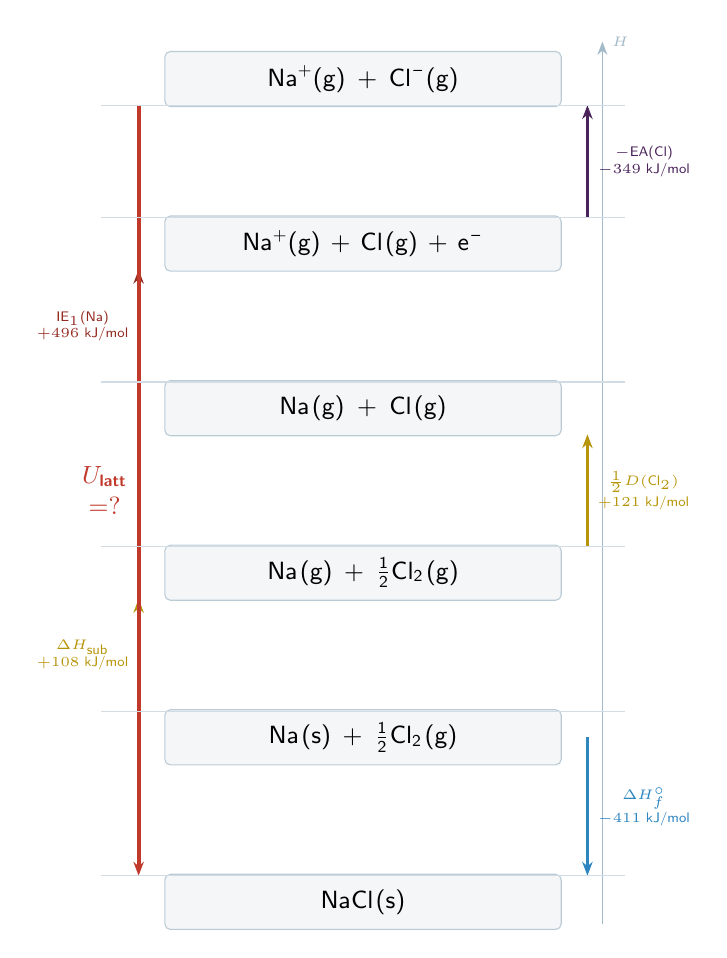
\begin{tikzpicture}[
  every node/.style={font=\sffamily\small, align=center},
  level/.style={draw=JourneyColor!30, fill=JourneyColor!5,
    minimum width=5.0cm, minimum height=0.7cm,
    rounded corners=2pt, text width=4.8cm},
  arr/.style={-{Stealth[length=5pt]}, thick},
  scale=0.95
]
  % Levels (right side = enthalpy axis)
  \node[level] (nacl_s) at (0, 0) {\ce{NaCl(s)}};
  \node[level] (na_cl_s) at (0, 2.2)
    {\ce{Na(s) + \frac{1}{2}Cl2(g)}};
  \node[level] (na_cl_g) at (0, 4.4)
    {\ce{Na(g) + \frac{1}{2}Cl2(g)}};
  \node[level] (na_clat_g) at (0, 6.6)
    {\ce{Na(g) + Cl(g)}};
  \node[level] (naion_cl_g) at (0, 8.8)
    {\ce{Na^+(g) + Cl(g) + e^-}};
  \node[level] (ions_g) at (0, 11.0)
    {\ce{Na^+(g) + Cl^-(g)}};

  % Enthalpy axis
  \draw[-{Stealth}, thin, JourneyColor!40]
    (3.2, -0.3) -- (3.2, 11.5)
    node[right, font=\sffamily\tiny] {$H$};

  % Arrows with labels
  % Formation: NaCl(s) from elements, down arrow (exo)
  \draw[arr, ModuleColor] (3.0, 2.2) -- (3.0, 0.35)
    node[midway, right, font=\sffamily\tiny, text=ModuleColor]
      {$\Delta H_f^\circ$\\$-411$ kJ/mol};

  % Sublimation of Na
  \draw[arr, DiscoveryColor] (-3.0, 2.55) -- (-3.0, 4.05)
    node[midway, left, font=\sffamily\tiny, text=DiscoveryColor]
      {$\Delta H_\text{sub}$\\$+108$ kJ/mol};

  % Dissociation of Cl2
  \draw[arr, DiscoveryColor] (3.0, 4.75) -- (3.0, 6.25)
    node[midway, right, font=\sffamily\tiny, text=DiscoveryColor]
      {$\frac{1}{2}D(\text{Cl}_2)$\\$+121$ kJ/mol};

  % Ionisation of Na
  \draw[arr, IonicColor] (-3.0, 6.95) -- (-3.0, 8.45)
    node[midway, left, font=\sffamily\tiny, text=IonicColor]
      {IE$_1$(Na)\\$+496$ kJ/mol};

  % Electron affinity of Cl
  \draw[arr, ProblemColor] (3.0, 9.15) -- (3.0, 10.65)
    node[midway, right, font=\sffamily\tiny, text=ProblemColor]
      {$-$EA(Cl)\\$-349$ kJ/mol};

  % Lattice energy (big downward arrow, left side)
  \draw[arr, WarningColor, line width=1.5pt]
    (-3.0, 10.65) -- (-3.0, 0.35)
    node[midway, left, font=\sffamily\small\bfseries, text=WarningColor]
      {$U_\text{latt}$\\$= ?$};

  % Connecting horizontal lines
  \foreach \y in {0.35, 2.55, 4.75, 6.95, 9.15, 10.65} {
    \draw[thin, JourneyColor!20] (-3.5,\y) -- (3.5,\y);
  }

\end{tikzpicture}
\end{center}

\vspace{0.4em}

By Hess's law, the sum of all steps must equal zero
around the cycle:
\[
  \Delta H_f^\circ = \Delta H_\text{sub}(\text{Na})
  + \tfrac{1}{2}D(\text{Cl}_2)
  + \text{IE}_1(\text{Na})
  - \text{EA}(\text{Cl})
  + U_\text{latt}
\]

Rearranging:
\begin{align*}
  U_\text{latt}(\text{NaCl})
  &= \Delta H_f^\circ - \Delta H_\text{sub} - \tfrac{1}{2}D
     - \text{IE}_1 + \text{EA} \\
  &= (-411) - (108) - (121) - (496) + (349) \\
  &= \mathbf{-787\ \text{kJ/mol}}
\end{align*}

This agrees almost exactly with the electrostatic calculation
using the Madelung constant ($-788$ kJ/mol).
The ionic model is quantitatively correct for NaCl.

\vspace{0.5em}

The cycle reveals something important:
\emph{every step except lattice formation costs energy}.
\begin{itemize}[nosep, leftmargin=2em]
  \item Sublimating Na: $+108$ kJ/mol
  \item Dissociating \ce{Cl2}: $+121$ kJ/mol
  \item Ionising Na: $+496$ kJ/mol (large!)
  \item Electron affinity of Cl: $-349$ kJ/mol (helps)
\end{itemize}

The total cost of forming the gas-phase ions is
$+376$ kJ/mol.
The lattice energy ($-787$ kJ/mol) more than pays for this.
\textbf{Ionic compounds form because the lattice energy
is large enough to cover the ionisation energy.}

% ─── Properties from the ionic model ─────────────────────────────────────────
\subsection{Predicting Properties from Lattice Energy}

The magnitude of the lattice energy determines the
physical properties of an ionic compound.

\begin{center}
\small
\begin{tabular}{llccc}
\toprule
Compound & Structure & $r_0$ (pm) & Lattice energy (kJ/mol) & M.p.\ (\textdegree C) \\
\midrule
LiF  & rock salt & 201 & $-1037$ & 845 \\
NaF  & rock salt & 231 & $-923$  & 993 \\
KF   & rock salt & 267 & $-821$  & 858 \\
NaCl & rock salt & 281 & $-788$  & 801 \\
NaBr & rock salt & 298 & $-752$  & 747 \\
NaI  & rock salt & 323 & $-705$  & 661 \\
MgO  & rock salt & 210 & $-3795$ & 2852 \\
CaO  & rock salt & 240 & $-3414$ & 2613 \\
\bottomrule
\end{tabular}
\end{center}

\vspace{0.5em}

Trends:
\begin{itemize}[nosep, leftmargin=2em]
  \item \textbf{Larger ions} (NaF $\to$ NaI): lattice energy
        decreases as $r_0$ increases; melting point falls.
  \item \textbf{Higher charges} (NaCl vs MgO): MgO has
        charges $2+/2-$ vs $1+/1-$; lattice energy is
        $\sim 5\times$ larger; melting point nearly
        $3\times$ higher.
  \item The formula $U \propto z_+z_-/r_0$ predicts both trends.
\end{itemize}

% ─── Dissolving ionic compounds ───────────────────────────────────────────────
\subsection{Why Ionic Compounds Dissolve: The Hydration Cycle}

NaCl dissolves in water readily despite its large lattice energy.
The reason: water molecules are polar and surround each
ion with a \newterm{hydration shell}, releasing energy
comparable to the lattice energy.

\[
  \Delta H_\text{sol} = U_\text{latt} + \Delta H_\text{hyd}(\text{Na}^+)
                        + \Delta H_\text{hyd}(\text{Cl}^-)
\]

For NaCl:
\[
  \Delta H_\text{sol} = (+788) + (-406) + (-363) = +19\ \text{kJ/mol}
\]

The dissolution is slightly endothermic,
yet NaCl dissolves spontaneously because the entropy
gain (ions dispersing into solution) more than compensates.
For many salts (e.g.\ MgO), the lattice energy is so
large that neither hydration nor entropy can overcome it
--- MgO is essentially insoluble.

\begin{problembox}
\begin{enumerate}[label=\textbf{\arabic*.}]
  \item \textbf{Born-Haber cycle for MgCl$_2$.}

    Given the following data:
    \begin{center}
    \small
    \begin{tabular}{ll}
    \toprule
    Quantity & Value (kJ/mol) \\
    \midrule
    $\Delta H_f^\circ(\text{MgCl}_2, s)$ & $-641$ \\
    $\Delta H_\text{sub}(\text{Mg})$     & $+148$ \\
    $D(\text{Cl}_2)$ (full bond)          & $+242$ \\
    IE$_1$(\text{Mg})                    & $+738$ \\
    IE$_2$(\text{Mg})                    & $+1451$ \\
    EA(\text{Cl})                        & $+349$ \\
    \bottomrule
    \end{tabular}
    \end{center}
    \begin{enumerate}[label=(\alph*)]
      \item Draw the full Born-Haber cycle for \ce{MgCl2}.
            Note that two \ce{Cl} atoms are needed,
            and Mg loses two electrons.
      \item Calculate $U_\text{latt}(\text{MgCl}_2)$.
      \item Compare to the estimated value from
            the Kapustinskii approximation:
            \[
              U \approx \frac{120\,200\,\nu\,z_+z_-}{r_+\!+r_-}
              \left(1-\frac{34.5}{r_+\!+r_-}\right)
            \]
            where $\nu$ is the number of ions per formula unit,
            $r_+ = 72$ pm (Mg$^{2+}$), $r_- = 181$ pm (Cl$^-$),
            and all distances are in pm.
    \end{enumerate}

  \item \textbf{Lattice energy and compound stability.}

    \begin{enumerate}[label=(\alph*)]
      \item NaCl exists; NaCl$_2$ does not.
            The hypothetical compound NaCl$_2$ would contain
            Na$^{2+}$ (IE$_1+$IE$_2 = 496+4562$ kJ/mol).
            Estimate whether NaCl$_2$ would have a more
            or less negative lattice energy than NaCl
            (use the proportionality $U \propto z_+z_-/r_0$).
      \item Despite the higher lattice energy, NaCl$_2$ does not form.
            Calculate whether the Born-Haber cycle for
            NaCl$_2$ gives a net positive or negative
            $\Delta H_f^\circ$.
      \item What does this calculation tell you about why
            Group~1 metals form $1+$ ions rather than $2+$?
    \end{enumerate}

  \item \textbf{Trends in melting point.}

    The melting points (\textdegree C) of Group~2 oxides are:
    BeO (2578), MgO (2852), CaO (2613), SrO (2531), BaO (1923).
    \begin{enumerate}[label=(\alph*)]
      \item The ionic radii increase down the group:
            Be$^{2+}$ 45 pm, Mg$^{2+}$ 72 pm,
            Ca$^{2+}$ 100 pm, Sr$^{2+}$ 118 pm, Ba$^{2+}$ 135 pm.
            (O$^{2-}$ radius $= 140$ pm in all cases.)
            Use $U \propto 1/(r_+ + r_-)$ to predict the
            relative lattice energies.
      \item Does the melting point trend follow the
            lattice energy trend?
      \item BeO has an anomalously high melting point
            for its small size.
            Suggest a reason involving its high charge density
            and the covalent character of very small, highly
            charged cations.
    \end{enumerate}
\end{enumerate}
\end{problembox}

% ─── Model breaks ─────────────────────────────────────────────────────────────
\subsection*{Where the Ionic Model Breaks Down}

\begin{modelbreaks}
The ionic model (point charges, pure electrostatics) fails for:

\begin{itemize}[nosep, leftmargin=2em]
  \item \textbf{Covalent character in ``ionic'' compounds}.
        When a cation is small and highly charged
        (e.g.\ Al$^{3+}$, Be$^{2+}$), it strongly polarises
        the anion's electron cloud (\newterm{Fajans' rules}).
        The electron density is distorted toward the cation,
        introducing covalent character.
        AlCl$_3$ sublimes at $\SI{180}{\degreeCelsius}$ rather
        than melting at high temperature like a true ionic solid.

  \item \textbf{Polyatomic ions}.
        The Madelung calculation assumes spherical point charges.
        \ce{NO3-}, \ce{SO4^{2-}}, \ce{CO3^{2-}} are not
        spherical; their charge is delocalised over several atoms.
        The lattice energy calculation requires modification.

  \item \textbf{Defects and non-stoichiometry}.
        Real ionic crystals contain vacancies, interstitials,
        and substitutional defects.
        Iron(II) oxide is not exactly FeO but rather
        Fe$_{0.95}$O --- iron vacancies are common.
        The perfect lattice model ignores all of this.

  \item \textbf{Very small ions or very large charge differences}.
        For compounds like \ce{Li2O} or \ce{AlF3},
        the simple point-charge model gives lattice energies
        differing from experiment by 5--10\%.
\end{itemize}
\end{modelbreaks}

\subsection*{Deep Problems}

\begin{deepbox}
\begin{enumerate}[label=\textbf{D\arabic*.}]

  \item \textbf{Convergence of the Madelung series.}

    The Madelung constant for NaCl is:
    \[
      M = \sum_j \frac{(\pm 1)}{d_j}
    \]
    where $d_j = r_j/r_0$ is the reduced distance of the
    $j$th ion from the central ion.

    The shells around a central Na$^+$ in NaCl (rock salt):
    \begin{center}
    \small
    \begin{tabular}{lccc}
    \toprule
    Shell & Distance $d_j$ & Number & Charge sign \\
    \midrule
    1 & 1           & 6  & $-$ (Cl$^-$) \\
    2 & $\sqrt{2}$  & 12 & $+$ (Na$^+$) \\
    3 & $\sqrt{3}$  & 8  & $-$ (Cl$^-$) \\
    4 & 2           & 6  & $+$ (Na$^+$) \\
    5 & $\sqrt{5}$  & 24 & $-$ (Cl$^-$) \\
    6 & $\sqrt{6}$  & 24 & $+$ (Na$^+$) \\
    \bottomrule
    \end{tabular}
    \end{center}
    \begin{enumerate}[label=(\alph*)]
      \item Compute the partial Madelung sum through
            all six shells listed.
            How close are you to $M = 1.748$?
      \item Notice that the partial sums oscillate.
            In which direction does the series approach
            the limit from above or below?
      \item The alternating-sign series converges very slowly
            because each new shell is almost large enough
            to cancel the previous ones.
            Ewald summation converts this conditionally
            convergent real-space sum into a combination
            of two absolutely convergent series
            (one in real space, one in reciprocal space).
            Explain in one paragraph why rearranging
            a conditionally convergent series can change
            its sum (Riemann rearrangement theorem),
            and why this is physically dangerous for
            the Madelung calculation.
    \end{enumerate}

  \item \textbf{Designing a high-temperature ionic material.}

    Ceramic insulators used in jet engines must:
    (a) remain solid above \SI{1500}{\degreeCelsius},
    (b) be electrically insulating,
    (c) be chemically resistant.
    From the lattice energy arguments in this module,
    select and justify the best ionic compound from this list:
    NaCl, MgO, \ce{Al2O3}, \ce{ZrO2}, \ce{CaF2}.
    For each candidate, estimate or look up the melting point
    and explain the lattice energy contribution.
    Identify which compound is used in practice for thermal
    barrier coatings in aircraft turbines and why.

\end{enumerate}
\end{deepbox}

\subsection*{Reflection}

\begin{reflectionbox}
\begin{enumerate}[label=\textbf{R\arabic*.}]
  \item The Born-Haber cycle shows that forming Na$^+$ costs
    $+496$ kJ/mol, yet NaCl is stable.
    \textbf{Does this mean that ``ionisation'' is the wrong
    way to think about NaCl?}
    Is there a sense in which calling NaCl an ``ionic compound''
    is a convenient fiction rather than a physical reality?

  \item The Madelung series for NaCl converges to 1.748.
    This number encodes the geometry of the entire infinite
    crystal --- the positions of every ion out to infinity.
    \textbf{In what sense does a macroscopic property (melting point)
    depend on an infinite sum?}
    How does the mathematics of infinite sums enter physical reality?

  \item The hydration energy of Na$^+$ ($-406$ kJ/mol) is
    almost as large as the lattice energy per ion pair.
    \textbf{What does it mean that water ``knows''
    how to stabilise an ion almost as well as the crystal it came from?}
    Is the liquid state in general underrated as a chemical environment?
\end{enumerate}
\end{reflectionbox}

\vspace{1.5em}
\begin{center}
\begin{tcolorbox}[enhanced, colback=DiscoveryColor!8, colframe=DiscoveryColor,
  width=0.88\textwidth, arc=3pt]
\centering\sffamily\small
\textbf{What we invented in this module.}\\[4pt]
Ionic bonding is pure electrostatics applied to an infinite
array of point charges.
The Madelung constant captures the geometry of that array;
the Born-Haber cycle decomposes the overall stability into
measurable steps.
The key insight: ionic compounds form not because ionisation
is cheap, but because the lattice energy is large enough
to pay for ionisation and still leave the compound more
stable than its elements.
Lattice energy scales as $z_+z_-/r_0$: double the charge
and the energy quadruples; halve the ion separation and
it doubles. This single relationship explains why MgO melts
at nearly \SI{3000}{\degreeCelsius} while NaI melts at
\SI{661}{\degreeCelsius}.
\end{tcolorbox}
\end{center}

\vspace{2em}
\noindent\textcolor{JourneyColor!40}{\rule{\textwidth}{0.6pt}}
\begin{center}\textit{\sffamily\small
Module 4.2 complete. Continue to Module 4.3:\\
\textbf{Covalent Bonding: Orbitals Overlapping}.}
\end{center}
\end{document}